\documentclass[a4paper,11pt]{article}

\usepackage[english, portuguese]{babel}
%\usepackage[portuguese]{babel}
\usepackage[T1]{fontenc}
\usepackage{amsmath, amssymb}
\usepackage{graphicx}
\usepackage[utf8]{inputenc}
\usepackage{color}
\usepackage{listings}
\usepackage{cancel}

\lstset{
    backgroundcolor=\color[rgb]{0.86,0.88,0.93},
    language=matlab, keywordstyle=\color[rgb]{0,0,1},
    basicstyle=\footnotesize \ttfamily,breaklines=true,
    escapeinside={\%*}{*)}
}

\begin{document}

%%%%%%%%%% Title %%%%%%%%%%%
\begin{figure}[!h] 
\includegraphics [scale=0.3] {Course-name} \end{figure}
%\pagestyle{empty}
{\Large \noindent \bf Homework II} 

\vskip0.8cm

%%%%%%%%%% Content starts here %%%%%%%%%%%
{\Large \noindent \bf Exercise 1} \hfill					20 Points\\

\noindent The unit steps responses of two systems $A$ and $B$ are recorded and reported in the files {\tt HW2\_ex1\_dataA.txt} and  {\tt HW2\_ex1\_dataB.txt}, respectively. In each file, the first column gives the time vector $t$ and the second column gives the output response $y$. \\

\noindent It is required to:
\begin{enumerate}
\item Load the data in Matlab/Octave and plot the two responses.
\item Estimate the transfer functions for the system $A$ and $B$. 
\item Compare your estimated systems with the ones provided in the data.
\end{enumerate}

\vskip0.5cm

\subsection*{Solution 1}
\begin{enumerate}
	\item Imprimindo os gráficos:\\
	\begin{figure}[!h]  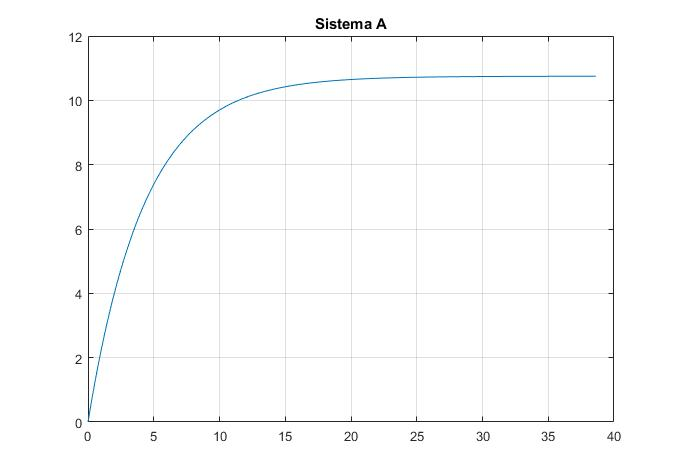
\includegraphics [scale=0.5] {Figures/systemA} \end{figure}
	\begin{figure}[!h]  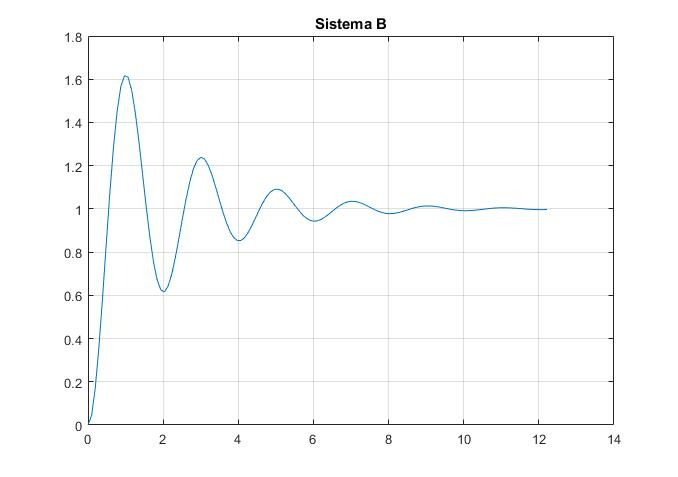
\includegraphics [scale=0.5] {Figures/systemB} \end{figure}
	\item \begin{itemize}
		\item Observando o gráfico do sistema A, concluímos que o mesmo é um sistema de primeira ordem. Portanto, $G_a(s) = \cfrac{k}{s+a} $.
		\\
		Para calcularmos $a$, fazemos que $T_s = \cfrac{4}{a}$, onde $T_s$ corresponde ao Tempo de estabilização, que é o tempo quando o sistema atinge 98\% do valor final. Como o valor final é 10.7486, então o tempo quando seu valor for 10.5336 será o $T_s$. Olhando pelos dados fornecidos, temos então que $16.8319 = \cfrac{4}{a}\longrightarrow a = 0.2376$.
		\vskip0.1cm
		Já o K, podemos calcular a partir do valor final, onde $V_\text{f}= \cfrac{K}{a}$. Como o Valor Final é 10.7486, teremos que
		\vskip0.1cm
		$K = 0.2376*10.7486\longrightarrow K=2.5543$
		\vskip0.1cm
		Sendo assim, $G_a(s) = \cfrac{K}{s+a}\longrightarrow \boxed{G_a(s) = \cfrac{2.5543}{s + 0.2376}}$
		\item Já no sistema B, podemos identificá-lo como um sistema de segunda ordem. Portanto, $G_b(s) = \cfrac{\omega_n^2}{s^2 +2\zeta \omega_n s+\omega_n^2}$, onde $\omega_n$ é a
		\vskip0.1cm
		frequência natural do sistema e $\zeta$ é taxa de amortecimento. Para calcular o $\zeta$, utilizamos a seguinte relação: $\zeta = \cfrac{-\ln\bigg(\cfrac{\%OS}{100}\bigg)}{\sqrt{\ln^2\bigg(\cfrac{\%OS}{100}\bigg) + \pi^2}} $, onde $\%OS$ é a porcentagem de \textit{overshoot}, que é quanto foi ultrapassado o valor final do sistema. Essa porcentagem é calculada através da razão $\%OS = \cfrac{C_\text{max} - C_\text{final}}{C_\text{final}} * 100$. Com isso, temos que $\zeta = 0.1498 $. Para calcularmos o $\omega_n$, utilizamos o Tempo de pico, que nada mais é do que o tempo no qual o valor máximo foi alcançado. Conseguimos identificar que o valor máximo foi 1.6165 e, verificando na tabela de dados, seu tempo de pico será 0.9695. Então, através da relação $\omega_n=\cfrac{\pi}{T_p\sqrt{1-\zeta}}$ achamos que $\omega_n = 3.2774 $. Com isso, chegamos que $G_b(s) = \cfrac{\omega_n^2}{s^2 +2\zeta \omega_n s+\omega_n^2} \longrightarrow\\ \boxed{G_b(s) = \cfrac{10.7415}{s^2 + 0.9822s + 10.7415}}$
	\end{itemize}
\item Gráficos comparativos:
	\begin{figure}[!h]  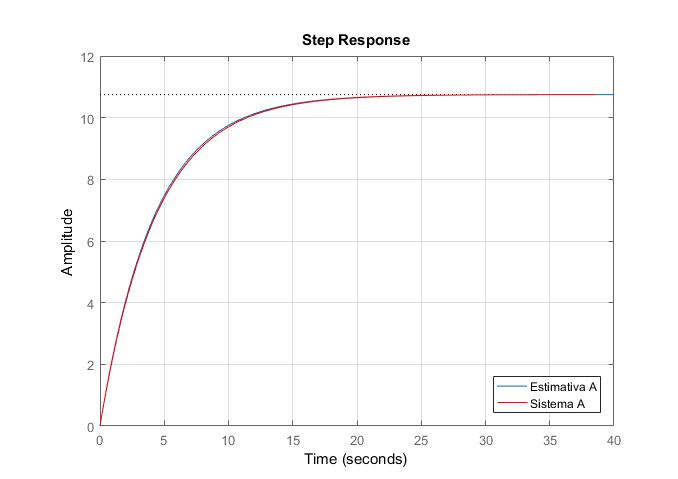
\includegraphics [scale=0.5] {Figures/systemAcomparison} \end{figure}
	\newpage 
	\begin{figure}[!h]  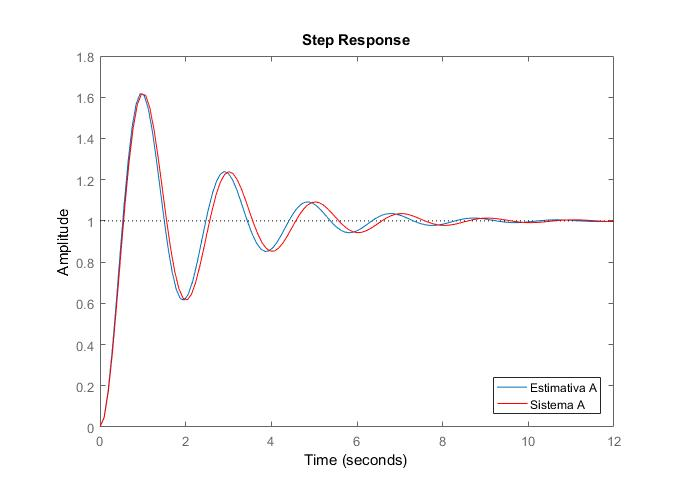
\includegraphics [scale=0.5] {Figures/systemBcomparison} \end{figure}
\end{enumerate}

\begin{lstlisting}
%% Exercise 1
Clear all; clc;

[Xa,Ya] = textread('HW2_ex1_dataA.txt','%f %f');
[Xb,Yb] = textread('HW2_ex1_dataB.txt','%f %f');

%% 1.1 
figure(1);
plot(Xa,Ya)
grid on
title('Sistema A')

figure(2);
plot(Xb,Yb)
grid on
title('Sistema B')

%% 1.3
a = 4/Xa(86)
k = a*Ya(196)
numa = [ k ]
dena = [ 1 a]
Ga = tf(numa,dena)
figure(3)
step(Ga); hold on;
plot(Xa,Ya,'color','r')
grid on;
legend('Estimativa A','Sistema A','Location','southeast')

OS = (max(Yb)-Yb(127))/Yb(127)*100
damp = -log(OS/100)/sqrt((log(OS/100)^2)+pi^2)
wn = pi/(Xb(11)*sqrt(1-damp^2))
numb = [ wn^2 ]
denb = [ 1 2*damp*wn wn^2]
Gb = tf(numb, denb)
figure(4)
step(Gb); hold on;
plot(Xb,Yb,'color','r')
legend('Estimativa A','Sistema A','Location','southeast')
\end{lstlisting}
\vskip0.4cm

{\Large \noindent \bf Exercise 2} \hfill					25 Points\\

\noindent Find the transfer function, $T(s)=C(s)/R(s)$, for the system in Figure (\ref{fig:ex2}), using the following methods:

\begin{enumerate}
\item Block diagram reduction.
\item Matlab/Octave. Use the following transfer functions:
\begin{align*}
G1(s)& =\cfrac{1}{(s+7)}, \quad G2(s)=\cfrac{1}{(s^2 + 2 s+3)},\\
G3(s)& =\cfrac{1}{(s+4)}, \quad G4(s) =\cfrac{1}{s},\\
G5(s)& =\cfrac{5}{(s+ 7)}, \quad G6(s) =\cfrac{1}{(s^2 + 5s + 10)},\\
G7(s)&= \cfrac{3}{(s+ 2)}, \quad G8(s) = \cfrac{1}{(s + 6)}. 
\end{align*}
{\bf Hint}: Use the {\tt append} and {\tt connect} commands in Matlab/Octave Control System Toolbox/Package.
\end{enumerate}

\begin{figure}[ht!] \begin{center}
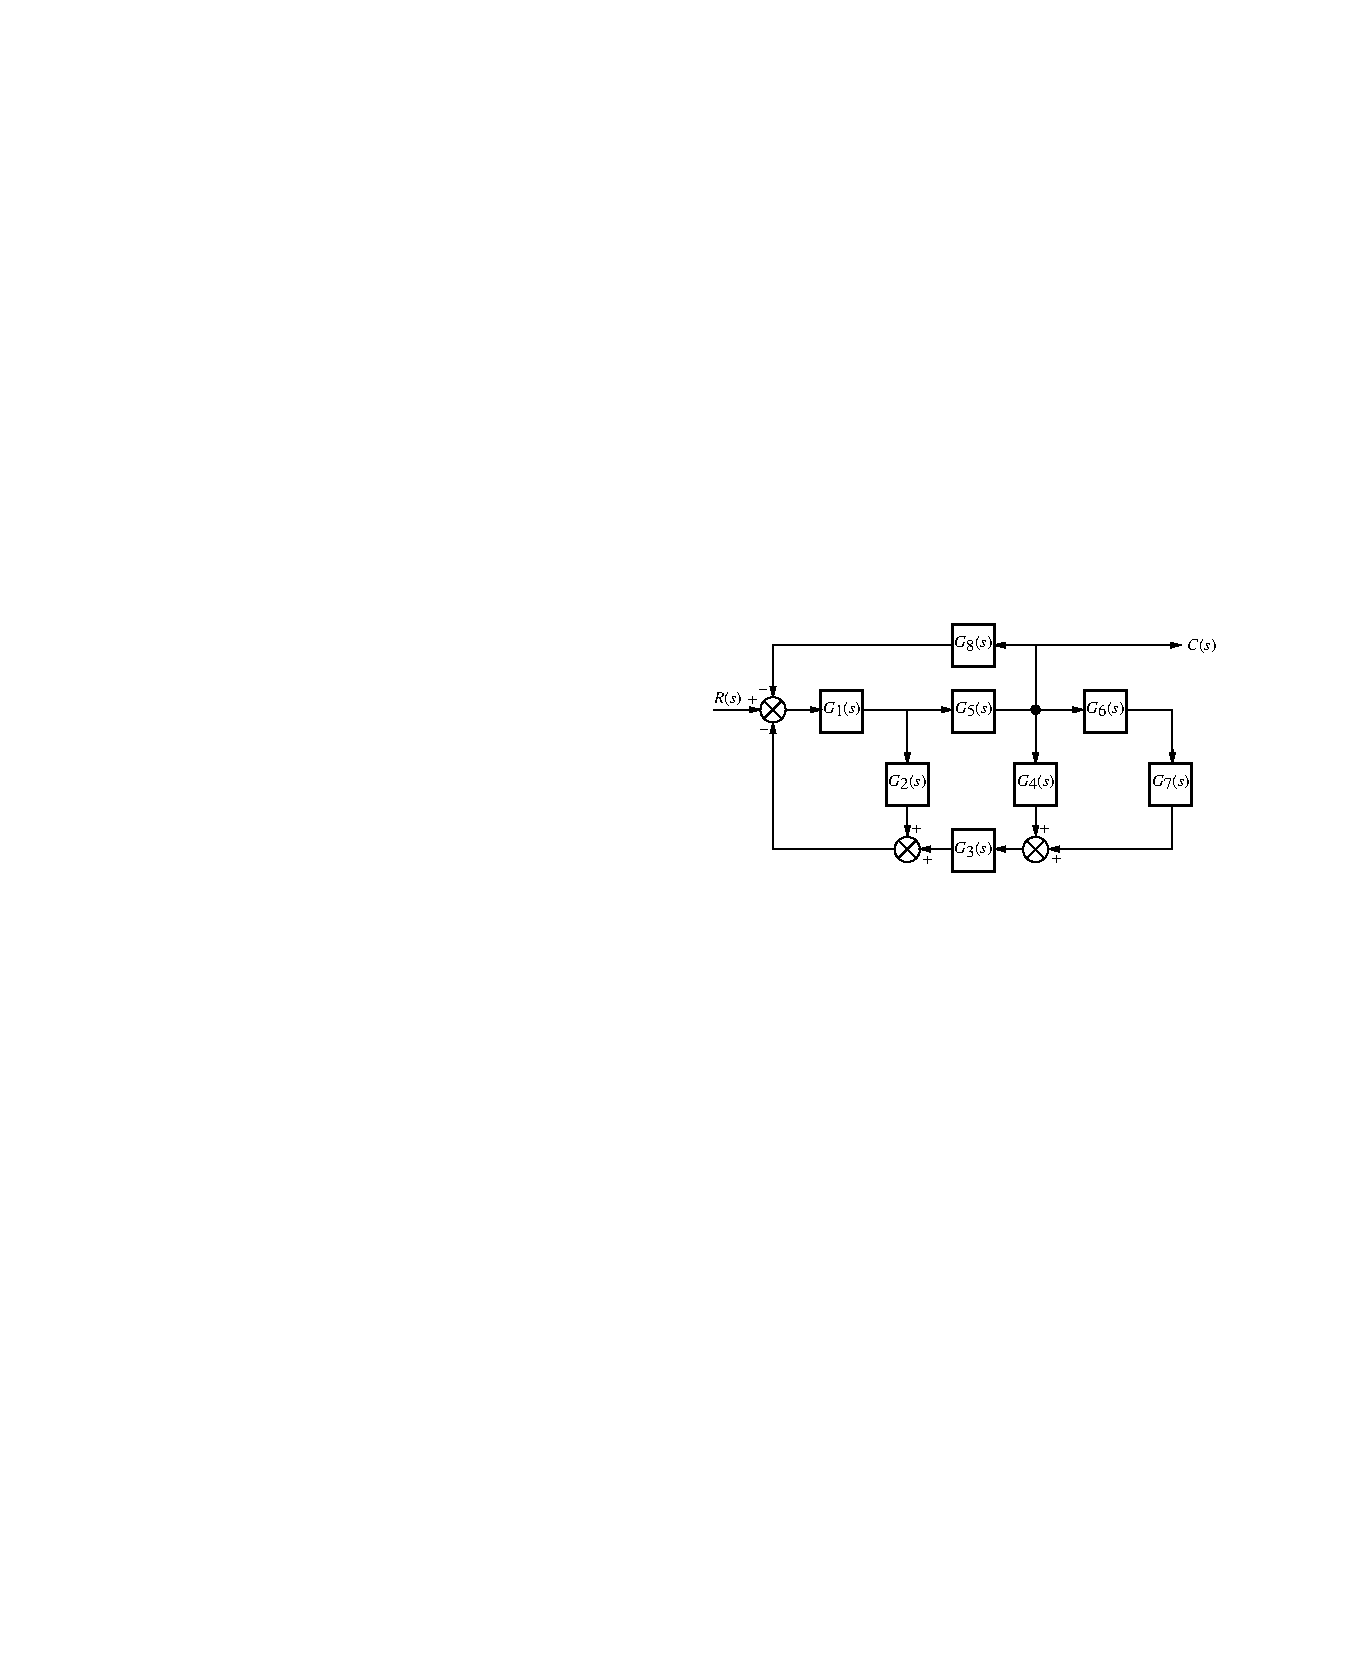
\includegraphics[width=1\textwidth]{Figures/blocks_ex}
 \caption{Block diagram for Exercise 2.} \label{fig:ex2}
\end{center} \end{figure}
\newpage
\vskip0.5cm
\subsection*{Solution 2}
\begin{enumerate}
	\item Após utilizar as propriedades de soma e concatenação de blocos chegamos no bloco com a função de transferência \\$G(s) = \cfrac{G_1(s)G_5(s)}{1+G_1(s)[[G_2(s)+G_5(s)G_3(s)[G_4(s)+G_6(s)G_7(s)]]+G_8(s)G_5(s)]}$
	\item 
	\begin{lstlisting}
	s = tf('s');
	G1= 1/(s+7); G2= 1/(s^2+2*s+3);
	G3= 1/(s+4); G4= 1/s;
	G5= 5/(s+7); G6= 1/(s^2+5*s+10);
	G7= 3/(s+2); G8= 1/(s+6);
	
	Gm = (G1*G5)/(1+G1*(G2+G3*G5*(G4+G6*G7)+G5*G8))
	
	Sum1 = sumblk('b = r - a - d');
	Sum2 = sumblk('d = f + g');
	Sum3 = sumblk('h = i + j');
	
	G1.u = 'b'; G1.y = 'e';
	G2.u = 'e'; G2.y = 'f';
	G3.u = 'h'; G3.y = 'g';
	G4.u = 'c'; G4.y = 'i';
	G5.u = 'e'; G5.y = 'c';
	G6.u = 'c'; G6.y = 'k';
	G7.u = 'k'; G7.y = 'j';
	G8.u = 'c'; G8.y = 'a';
	
	Ss = connect(G1,G2,G3,G4,G5,G6,G7,G8,Sum1,Sum2,Sum3,'r','c');
	
	[num, den] = ss2tf(Ss.A,Ss.B,Ss.C,Ss.D);
	Gs = tf(num,den)
	figure(1)
	step(Gs,'r',Gm,'b'); grid on;
	legend('Simulado','Manual');
	\end{lstlisting}
	\begin{figure}[!h]  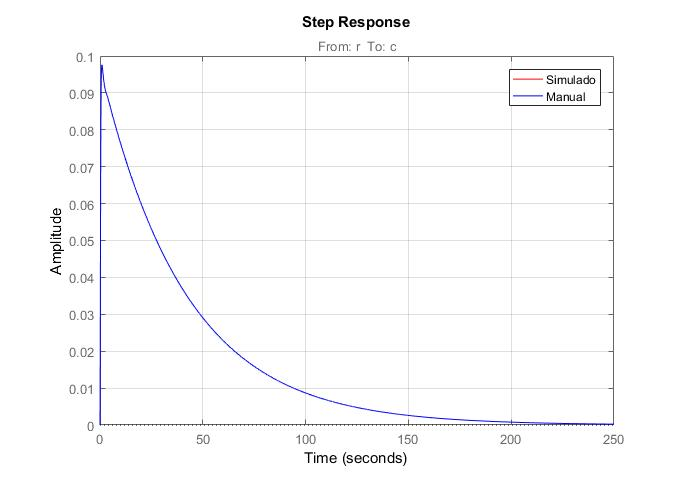
\includegraphics [scale=0.5] {Figures/exercise2} \end{figure}
	P.S 1: Simulado refere-se ao calculado no MATLAB, enquanto manual refere-se ao feito por diagrama de blocos.\\
	P.S 2: O gráfico do simulado não aparece visível pois a linha do manual está sobrepondo totalmente ela. Contudo, através do MATLAB, pode ser verificado a semelhança entra as funções de transferência.\\
	P.S 3: Os valores concretos das funções de transferência foram omitidos devido ao seu tamanho exageradamente grande. Contudo, as variáveis Gs e Gm indicam as funções de transferência feita no MATLAB e através do diagrama de blocos, respectivamente.
\end{enumerate}
\vskip0.4cm

{\Large \noindent \bf Exercise 3} \hfill					20 Points\\

\noindent The system in state space given in (\ref{eq:ss}) represents the forward path of a unity feedback system. 
\begin{align}
\begin{split}
\mathbf{\dot{x}} & =\begin{bmatrix}
0 & 1 & 0\\
0 & 0 & 1\\
-3 & -4 & -5\\
\end{bmatrix}
\mathbf{x}+\begin{bmatrix}
0 & 0 & 1
\end{bmatrix}
u \\
y & = \begin{bmatrix}
0 & 1 & 1
\end{bmatrix}
\mathbf{x}
\end{split}
\label{eq:ss}
\end{align}

\noindent Constructing the Routh table in Matlab/Octave, use the Routh-Hurwitz criterion to determine if the closed loop is stable.

\vskip0.5cm

\subsection*{Solution 3}
\begin{lstlisting}
A = [0 1 0; 0 0 1; -3 -4 -5];
B = [0; 0; 1];
C = [0 1 1];
D = 0;

[num, den] = ss2tf(A,B,C,D);
T = tf(num,den);
G = feedback(T,1);

den = G.den;
s3 = [1 5 0];
s2 = [6 3 0];
s1 = [-det([s3(1) s3(2);s2(1) s2(2)])/s2(1) ...
-det([s3(1) s3(3);s2(1) s3(3)])/s2(2) 0];
s0 = [-det([s2(1) s2(2);s1(1) s1(2)])/s1(1) ...
-det([s2(1) s2(3);s1(1) s1(3)])/s1(2) 0];
s0(isnan(s0))=0;
R = [s3(1) s2(1) s1(1) s0(1)]


R =

1.0000    6.0000    4.5000    3.0000
\end{lstlisting}
Como não há troca de sinal entre as variáveis $S_n(0)$, concluímos que o sistema é estável.
\vskip0.4cm

{\Large \noindent \bf Exercise 4} \hfill					35 Points\\

\noindent  For a system with the state and output equations given in (\ref{eq:ex3}):
\begin{align}
\begin{split}
\dot{x}(t)& =x^2(t)-u(t)x(t)-2u(t)\\
y(t)& =x^3(t)+u^3(t)
\end{split}
\label{eq:ex3}
\end{align}  

\begin{enumerate}
\item Calculate the state and output equilibrium points when $u(t)=u_{eq}=1$.
\item Define the linearised system around the equilibrium points and analise the stability of the system.
\item \label{ex3:item3} Compare the linearised and nonlinear system responses $\delta y(t)$ for an input $\delta u(t)=A cos(2t)$, with $A=0.1$ applied at $t=0$.
\item \label{ex3:item4} {\bf Extra (5 points)}: Investigate how the responses differ when the input amplitude assumes the values $[0.05, 0.15, 0.2]$. 
\item {\bf Extra (5 points)}: Calculate the error between linearised and nonlinear system in point (\ref{ex3:item3}) and point (\ref{ex3:item4}). Comment your findings.
\end{enumerate}

\noindent{\bf Hint}: Use the command {\tt ode45} to simulate the nonlinear system.
\subsection*{Solution 4}
\begin{enumerate}
	\item No ponto de equilíbrio, temos que $\dot{x}(t)=0$. Logo, como $u(t)=u_{eq}=1$, chegamos nas seguintes equações:
	\begin{itemize}
		\item $x^2(t)-x(t)-2=0$
		\item $y(t)=x^3(t)+1$
	\end{itemize}
	Resolvendo a primeira equação, chegamos no seguinte resultado: 
	\begin{align*}
	x_1(t)=&2& 
	x_2(t)=&{-1}&
	\end{align*}
	Consequentemente, temos que a segunda equação fica:
	\begin{align*}
	y_1(t)=&2^3+1=9&\\
	y_2(t)=&{-1}^3+1=0&
	\end{align*}
	Sendo assim, os pontos de equilíbrio são:
	\begin{enumerate}
		\item 
		\begin{align*}
		x_1(t)=&2 &y_1(t)=&9
		\end{align*}
		\item 
		\begin{align*}
		x_2(t)=&{-1} &y_2(t)=&0
		\end{align*}
	\end{enumerate}
	\item Como temos 2 pares de pontos de equilibrio, resolvemos uma de cada vez:
	\begin{enumerate}
		\item
		\begin{align*}
		\dot{x}(t)=&x^2(t)-u(t)x(t)-2u(t)&
		y(t)=&x^3(t)+u^3(t)&\\
		&\text{Ponto de equilibrio}=(x_0,u_0)=(2,1)
		\end{align*}
		Usando série de Taylor para linearizarmos o sistema:
		\vskip0.1cm
		$$\cancel{\dot{x}_0(t)}+\Delta\dot{x}=\cancel{f(x_0,u_0)}+\cfrac{\partial f}{\partial x}\bigg\rvert_{(x_0,u_0)}.\Delta x+\cfrac{\partial f}{\partial u}\bigg\rvert_{(x_0,u_0)}.\Delta u $$
		\vskip0.1cm
		$$\Delta\dot{x}=(2\cancelto{2}{x(t)}-\cancelto{1}{u(t)})\bigg\rvert_{(x_0,u_0)}.\Delta x+(0-\cancelto{2}{x(t)}-2)\bigg\rvert_{(x_0,u_0)}.\Delta u$$
		\vskip0.1cm
		$$ \Delta\dot{x}=3\Delta x-4\Delta u\xrightarrow{\Delta x\triangleq x(t),\Delta u\triangleq u(t)}\boxed{\dot{x}(t)=3x(t)-4u(t)}$$
		\newpage
		$$\Delta y= \cfrac{\partial f}{\partial x}\bigg\rvert_{(x_0,u_0)}.\Delta x+\cfrac{\partial f}{\partial u}\bigg\rvert_{(x_0,u_0)}.\Delta u$$
		\vskip0.1cm
		$$\Delta y=(3x^2(t))\bigg\rvert_{(x_0,u_0)}.\Delta x+(3u^2(t))\bigg\rvert_{(x_0,u_0)}.\Delta u $$
		\vskip0.1cm
		$$ \Delta y=12\Delta x+3\Delta u\xrightarrow{\Delta x\triangleq x(t),\Delta u\triangleq u(t)}\boxed{y(t)=12x(t)+3u(t)} $$
		\vskip0.1cm
		Com as equações de estado e resposta conseguimos achar a função de transferência fazendo a transformada de Laplace:
		\begin{align*}
		sX(s)=&3X(s)-4U(s)&Y(s)=&12X(s)+3U(s)&
		\end{align*}
		Da primeira equação, temos:\\
		$$ X(s)=\cfrac{-4U(s)}{s-3}\xrightarrow[\text{segunda eq.}]{\text{Aplicando na}}Y(s)=\cfrac{-48U(s)}{s-3}+3U(s) $$
		\vskip0.1cm
		$$G(s)=\cfrac{Y(s)}{U(s)}=\cfrac{3s-57}{s-3}$$
		\vskip0.1cm
		Colocando em closed-loop para calcular a estabilidade:
		\vskip0.1cm
		$$ G(s)=\cfrac{G(s)}{1+G(s)}\longrightarrow \boxed{G(s)=\cfrac{3s-57}{4s-60}} $$
		\vskip0.1cm
		Sendo assim, o único polo será 15, que é do lado direito do plano real, caracterizando um sistema \textbf{instável}.
		\item 
		\begin{align*}
		\dot{x}(t)=&x^2(t)-u(t)x(t)-2u(t)&
		y(t)=&x^3(t)+u^3(t)&\\
		&\text{Ponto de equilibrio}=(x_0,u_0)=(-1,1)
		\end{align*}
		Usando série de Taylor para linearizarmos o sistema:
		\vskip0.1cm
		$$\cancel{\dot{x}_0(t)}+\Delta\dot{x}=\cancel{f(x_0,u_0)}+\cfrac{\partial f}{\partial x}\bigg\rvert_{(x_0,u_0)}.\Delta x+\cfrac{\partial f}{\partial u}\bigg\rvert_{(x_0,u_0)}.\Delta u $$
		\vskip0.1cm
		$$\Delta\dot{x}=(2\cancelto{-1}{x(t)}-\cancelto{1}{u(t)})\bigg\rvert_{(x_0,u_0)}.\Delta x+(0-\cancelto{-1}{x(t)}-2)\bigg\rvert_{(x_0,u_0)}.\Delta u$$
		\vskip0.1cm
		$$ \Delta\dot{x}=-3\Delta x-\Delta u\xrightarrow{\Delta x\triangleq x(t),\Delta u\triangleq u(t)}\boxed{\dot{x}(t)=-3x(t)-u(t)}$$
		\vskip0.1cm
		$$\Delta y= \cfrac{\partial f}{\partial x}\bigg\rvert_{(x_0,u_0)}.\Delta x+\cfrac{\partial f}{\partial u}\bigg\rvert_{(x_0,u_0)}.\Delta u$$
		\vskip0.1cm
		$$\Delta y=(3x^2(t))\bigg\rvert_{(x_0,u_0)}.\Delta x+(3u^2(t))\bigg\rvert_{(x_0,u_0)}.\Delta u $$
		\vskip0.1cm
		$$ \Delta y=3\Delta x+3\Delta u\xrightarrow{\Delta x\triangleq x(t),\Delta u\triangleq u(t)}\boxed{y(t)=3x(t)+3u(t)} $$
		\vskip0.1cm
		Com as equações de estado e resposta conseguimos achar a função de transferência fazendo a transformada de Laplace:
		\begin{align*}
		sX(s)=&-3X(s)-U(s)&Y(s)=&3X(s)+3U(s)&
		\end{align*}
		Da primeira equação, temos:\\
		$$ X(s)=\cfrac{-U(s)}{s+3}\xrightarrow[\text{segunda eq.}]{\text{Aplicando na}}Y(s)=\cfrac{-3U(s)}{s+3}+3U(s) $$
		\vskip0.1cm
		$$G(s)=\cfrac{Y(s)}{U(s)}=\cfrac{3s+6}{s+3}$$
		\vskip0.1cm
		Colocando em closed-loop para calcular a estabilidade:
		\vskip0.1cm
		$$ G(s)=\cfrac{G(s)}{1+G(s)}\longrightarrow \boxed{G(s)=\cfrac{3s+6}{4s+9}} $$
		\vskip0.1cm
		Sendo assim, o único polo será -2.25, que é do lado esquerdo do plano real, caracterizando um sistema \textbf{estável}.
	\end{enumerate}
	
	\item
\end{enumerate}
\newpage
\begin{lstlisting}
%% Exercise 4

% Item 2
num1=[3 -57];
den1=[1 -3];
temp= tf(num1,den1);
tf1 = feedback(temp,1)
pole1 = pole(tf1)

num2=[3 6];
den2=[1 3];
temp=tf(num2,den2);
tf2 = feedback(temp,1)
pole2 = pole(tf2)

\end{lstlisting}
\end{document}